% ══════════════════════════════════════════════════════════════════════════════
%  CAPITOLO — PROIEZIONI 2026-2031
%  Etichette: ch:forecast, sec:fc_data, sec:fc_models, sec:fc_choice,
%             sec:fc_volume, sec:fc_type, sec:fc_donors, sec:fc_summary
% ══════════════════════════════════════════════════════════════════════════════

\chapter{Proiezioni 2026--2031}
\label{ch:forecast}

Il \cref{ch:eda} ha mostrato un volume donazionale in contrazione del $28\%$ in
diciassette anni, con ingressi in calo e intensità individuale ferma; il
\cref{ch:retention} ha quantificato quanto rapidamente si perdono i donatori
dopo il primo contatto. Questa appendice proietta quegli andamenti in avanti di
sei anni, dal 2026 al 2031, per rispondere a una domanda operativa: quante
donazioni può ragionevolmente attendersi il sistema, e con quale margine di
incertezza.

A differenza del \cref{ch:glm}, che modella il comportamento del singolo
donatore per spiegare chi dona di più e perché, qui l'unità di analisi è il
volume aggregato e l'obiettivo non è inferenziale ma predittivo.

% ───────────────────────────────────────────────────────────────────────
\section{Serie storica e criterio di valutazione}
\label{sec:fc_data}

La serie di base è il conteggio mensile 2009--2025 ottenuto per aggregazione
diretta del dataset finale: 204 mesi per \textbf{353\,671 donazioni}
(\cref{fig:fc_monthly}). La struttura è quella descritta nella
\cref{sec:temporal} --- trend decrescente non lineare, stagionalità mensile
contenuta, uno shock esogeno di ampiezza modesta nel 2020.

\begin{figure}[H]
    \centering
    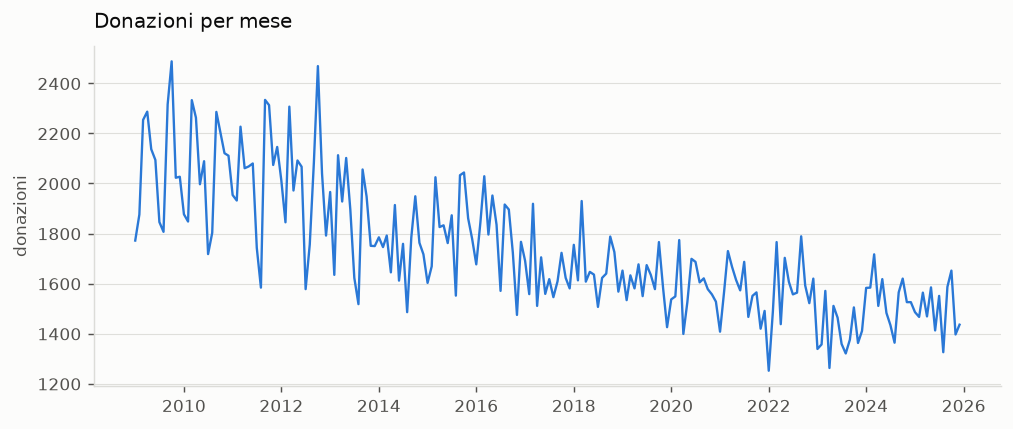
\includegraphics[width=0.95\linewidth]{img/fig_forecast_monthly_history.png}
    \caption{Serie mensile delle donazioni, 2009--2025.}
    \label{fig:fc_monthly}
\end{figure}

\paragraph{Come si confrontano i modelli.}
Il criterio adottato è un \textbf{backtest a origine mobile}: si sceglie un
anno origine $O$, si stima ogni modello sui soli dati fino a $O$, si prevedono
gli anni successivi e si confronta con l'osservato; poi si sposta l'origine in
avanti e si ripete. Con nove origini e orizzonti da uno a tre anni si ottengono
ventiquattro coppie (previsione, osservato) per ciascun candidato, tutte sugli
stessi anni bersaglio. L'orizzonte è limitato a tre anni perché è il massimo su
cui i modelli per donatore restano stimabili su tutte le origini; le baseline,
che non hanno questo vincolo, sono valutate a parte fino a sei anni --- ed è da
quel confronto, non da questo, che vengono la scelta di $\varphi$
(\cref{sec:fc_choice}) e gli intervalli empirici.

\paragraph{Come si produce una previsione.}
A ogni origine la previsione è \emph{a più passi}: il modello, stimato una
volta sui dati fino a $O$, produce in un colpo solo i valori di
$O+1, \dots, O+h^*$, senza essere aggiornato con l'osservato degli anni
intermedi (la previsione del 2019 fatta dall'origine 2016 non sa nulla del
2017 e del 2018, per esempio). Il metodo di estrapolazione dipende dalla famiglia
(\cref{sec:fc_models}). Le \textbf{baseline} sono formule chiuse sulla serie
annuale: la naive ripete l'ultimo anno, il trend smorzato prolunga una retta
stimata sulla storia con pendenza decrescente (\cref{eq:damped}). Il
\textbf{GLM mensile} prevede i $12h^*$ mesi successivi prolungando il termine
di trend e ripetendo il profilo stagionale stimato, e i mesi si sommano per
anno solare. I \textbf{modelli per donatore} non prevedono il totale ma lo
costruiscono: partendo dallo stato di ogni donatore a fine $O$, si simula un
anno alla volta quante volte ciascuno dona; l'esito simulato di un anno
aggiorna le covariate dell'anno successivo (tempo dall'ultima donazione, anni
di carriera) e ad ogni anno si aggiunge un contingente di nuovi donatori, la cui
numerosità è prevista a parte con un trend smorzato sulla serie degli
ingressi. Il totale che ne risulta è la media di venti percorsi simulati.

La procedura è riassunta nell'\cref{alg:backtest}. Il punto che conta è la
riga~4: la storia passata a ogni modello si ferma all'origine, quindi nessuna
previsione può usare informazione che al momento di produrla non esisteva. È la
sola garanzia che gli errori misurati siano errori di previsione e non di
adattamento.

\begin{algorithm}[H]
\caption{Backtest a origine mobile con finestra espansiva}
\label{alg:backtest}
\begin{algorithmic}[1]
\Require serie $y_{1:T}$; insieme di modelli $\mathcal{M}$; addestramento minimo
$m$; orizzonte massimo $H$
\Ensure una riga $(\text{modello}, O, h, y, \hat{y})$ per ogni valutazione
\State $R \gets \emptyset$
\For{$O = m$ \textbf{fino a} $T-1$}
  \Comment{ogni anno utilizzabile diventa un'origine}
  \State $\text{storia} \gets y_{1:O}$
  \Comment{\textbf{solo} il passato: qui si evita il leakage}
  \ForAll{$f \in \mathcal{M}$}
    \State $\hat{y}_{1:h^*} \gets f(\text{storia},\ h^*)$ \quad con
    $h^* = \min(H,\ T-O)$
    \For{$h = 1$ \textbf{fino a} $h^*$}
      \State $R \gets R \cup \{(f,\ O,\ h,\ y_{O+h},\ \hat{y}_h)\}$
    \EndFor
  \EndFor
\EndFor
\State \Return $R$
\Comment{MAPE, bias e percentili si aggregano da $R$, per modello o per orizzonte}
\end{algorithmic}
\end{algorithm}

\begin{table}[H]
\centering
\small
\caption{Simboli dell'\cref{alg:backtest} e valori adottati.}
\label{tab:backtest_simboli}
\begin{tabularx}{\linewidth}{@{}l X l@{}}
\toprule
\textbf{Simbolo} & \textbf{Significato} & \textbf{Valore} \\
\midrule
$y_t$ & donazioni osservate nell'anno $t$ & --- \\
$y_{1:T}$ & serie annuale completa & 2009--2025 \\
$T$ & numero di anni della serie & 17 \\
$\mathcal{M}$ & insieme dei modelli candidati & 17 \\
$f$ & un modello di $\mathcal{M}$: riceve la storia e un orizzonte, restituisce le previsioni & --- \\
$m$ & addestramento minimo, in anni, prima della prima origine & 8 \\
$H$ & orizzonte massimo di previsione & 3 (6 baseline) \\
$O$ & origine: ultimo anno usato per la stima & 2016--2024 \\
storia & dati disponibili all'origine, $y_{1:O}$ & --- \\
$h$ & orizzonte: distanza in anni dall'origine & $1,\dots,h^*$ \\
$h^*$ & orizzonte effettivo $\min(H,\,T-O)$, ridotto per le ultime origini & 3, 2 o 1 \\
$\hat{y}_h$ & previsione per l'anno $O+h$ fatta all'origine $O$ & --- \\
$y_{O+h}$ & valore osservato nello stesso anno & --- \\
$R$ & insieme dei risultati, una riga per valutazione & 24 per modello \\
\bottomrule
\end{tabularx}
\end{table}

Poiché ogni modello riceve le stesse origini e gli stessi bersagli, il confronto
della \cref{tab:fc_backtest} non dipende da quale periodo sia capitato a chi.
Dallo stesso insieme $R$ si ricavano, filtrando sul modello adottato e
raggruppando per orizzonte, i percentili che formano gli intervalli della
\cref{sec:fc_choice}.

La differenza rispetto a una singola divisione non è pedanteria. Con una sola
divisione il giudizio dipende da quale periodo è finito nel campione di
verifica: se contiene un evento eccezionale, si sta misurando quanto un modello
è fortunato, non quanto è accurato. Con nove origini l'evento eccezionale entra
in alcune finestre e non in altre, e il confronto diventa informativo. Va
segnalato che questo criterio è più severo del precedente: gli errori riportati
qui sotto sono più alti di quelli che si otterrebbero su un holdout singolo
favorevole, e sono la stima onesta.

% ───────────────────────────────────────────────────────────────────────
\section{Confronto tra approcci di modellazione}
\label{sec:fc_models}

Sono stati confrontati diciassette candidati, divisi in tre famiglie che
differiscono per ciò che modellano. Le \textbf{baseline} (nove) lavorano sulla
serie annuale con formule elementari: ultimo anno ripetuto, media degli ultimi
tre o cinque anni, trend lineare, trend smorzato con $\varphi \in \{0{,}6;\
0{,}7;\ 0{,}8\}$ e una media fra trend smorzato e media mobile. I
\textbf{modelli sulla serie aggregata} (due) sono GLM quasi-Poisson sulla serie
mensile, con effetti di mese e un trend lineare o a spline, e le previsioni
mensili si sommano per anno. I \textbf{modelli per singolo donatore} (sei) non
sono modelli di serie storiche: sono regressioni per conteggi sul panel
donatore-anno --- Poisson, binomiale negativa, hurdle, con e senza trend, e un
LightGBM con perdita di Poisson --- e il totale annuo si ottiene simulando ogni
donatore e sommando (\cref{sec:fc_data}). La \cref{tab:fc_backtest} riporta i
principali.

\begin{table}[ht]
\centering
\caption{Backtest a origine mobile: nove origini, scala annuale, orizzonti
da uno a tre anni. MAPE è l'errore percentuale medio assoluto, il bias l'errore
medio \emph{con segno} (negativo = sottostima).}
\label{tab:fc_backtest}
\begin{tabular}{@{}lrr@{}}
\toprule
\textbf{Modello} & \textbf{MAPE} & \textbf{Bias} \\
\midrule
\textbf{Trend lineare smorzato} ($\varphi = 0{,}6$) & $\mathbf{3{,}55\%}$ & $-0{,}8\%$ \\
GLM quasi-Poisson mensile, trend lineare            & $3{,}91\%$ & $-2{,}5\%$ \\
Trend lineare non smorzato                          & $4{,}92\%$ & $-4{,}1\%$ \\
Naive (ultimo anno osservato)                       & $5{,}17\%$ & $+3{,}7\%$ \\
Poisson per donatore, simulato e sommato            & $6{,}46\%$ & $+3{,}1\%$ \\
\emph{GLM quasi-Poisson mensile, spline a 4 gdl}    & $7{,}07\%$ & $-1{,}0\%$ \\
\bottomrule
\end{tabular}
\end{table}

\paragraph{GLM quasi-Poisson.}
Il \textbf{quasi-Poisson} è una variante della GLM di Poisson
(\cref{sec:glm_model}) che non specifica una distribuzione completa per la
risposta, ma soltanto i suoi primi due momenti~\cite{McCullaghNelder1989}:
\begin{equation}
    \mathbb{E}[\mathbf{Y}] = \mu, \quad \mathbb{V}[\mathbf{Y}] = \sigma^{2}\mu
\end{equation}
$\sigma^{2}$ è il \textbf{parametro di dispersione}: se $\sigma^{2} = 1$ si
ritrova la Poisson, se $\sigma^{2} > 1$ la varianza cresce in proporzione alla
media (\textbf{sovradispersione}). A differenza della binomiale negativa, in cui
la varianza cresce con il quadrato della media (\cref{eq:nb_var}), qui cresce
linearmente.
\newline
I coefficienti $\beta$ si stimano con le stesse equazioni della Poisson, quindi
\textbf{le stime puntuali coincidono}; $\sigma^{2}$ è stimato a parte con la
statistica di Pearson,
\begin{equation}
    \hat{\sigma}^{2} = \frac{1}{n-p}\sum_{i=1}^{n}
    \frac{(y_{i}-\hat{\mu}_{i})^{2}}{\hat{\mu}_{i}},
\end{equation}
con $n$ osservazioni e $p$ parametri, e gli errori standard vengono
moltiplicati per $\hat{\sigma}$. Non essendo definita una verosimiglianza, il
modello non ha AIC.
\newline
Per la previsione conta soltanto la media: il quasi-Poisson prevede quindi gli
stessi valori della Poisson, e la correzione riguarda solo l'incertezza sui
coefficienti. Il modello usato qui ha forma
\begin{equation}
    \ln \mu_{t} = \beta_{0} + f(\text{anno}_{t}) + \gamma_{m(t)},
    \label{eq:qp_form}
\end{equation}
dove $\mu_{t}$ è il numero atteso di donazioni nel mese $t$, $\gamma_{m(t)}$
l'effetto del mese dell'anno e $f$ il trend: lineare,
$f = \beta_{1}(\text{anno}_{t} - 2017)$, oppure una spline cubica a quattro
gradi di libertà.

Due risultati vanno isolati.

\paragraph{La spline è il problema.}
Il modello quasi-Poisson mensile con spline cubica a quattro gradi di libertà
sull'anno --- la forma che l'adattamento in campione premierebbe, e la scelta
naturale per una serie con un trend visibilmente non lineare --- sbaglia il
$7{,}07\%$. Sostituendo la spline con un semplice \textbf{termine
lineare sull'anno}, a parità di tutto il resto (stessa famiglia, stessi dati,
stesso codice, stesso fattore mensile; \cref{eq:qp_form}), l'errore
scende al $3{,}91\%$: si \emph{dimezza}.

La ragione è che la
curva stimata dalla spline è, dal 2015 in poi, indistinguibile da una retta.
Tutta la flessibilità dei quattro gradi di libertà è spesa sulla curvatura del
tratto 2009--2014, che per l'estrapolazione non serve; e la flessibilità che
non serve dentro il campione diventa instabilità fuori. È il difetto classico
di scegliere il termine di trend guardando l'adattamento anziché la previsione.

\paragraph{Il modello più semplice ha la meglio.}
Il candidato migliore è un \textbf{trend lineare smorzato}: si stima una retta
ai minimi quadrati sull'intera serie annuale disponibile all'origine, con
intercetta $a$ e pendenza $b$, e la si prolunga facendo decadere la pendenza
di un fattore $\varphi$ a ogni passo~\cite{GardnerMcKenzie1985}:
\begin{equation}
  \hat{y}_{O+h} = \ell_O + b \sum_{i=1}^{h} \varphi^{i},
  \qquad \ell_O = a + b\,(O - 2009),
  \label{eq:damped}
\end{equation}
dove $\ell_O$ è il valore della retta nell'anno origine. Per $\varphi = 1$ si
ritrova la retta non smorzata; per $\varphi < 1$ gli incrementi si
riducono geometricamente e la proiezione converge al livello
$\ell_O + b\,\varphi/(1-\varphi)$ invece di proseguire indefinitamente. È fra i
modelli più semplici del confronto e sbaglia meno di tutti gli altri.

Lo smorzamento non è un parametro scelto con il senno di poi: sul backtest delle
sole baseline a sei anni, tutto l'intervallo $\varphi \in [0{,}3;\ 0{,}9]$ produce MAPE fra $3{,}8\%$ e
$4{,}9\%$, mentre \emph{non} smorzare ($\varphi = 1$) costa $6{,}19\%$. L'importante
in questo caso è l'azione di smorzamento, non quanto vale $\varphi$.

Che modelli elementari battano modelli strutturati su orizzonti lunghi è un
esito noto nella letteratura previsiva~\cite{GardnerMcKenzie1985,Tashman2000}: 
per ogni sessennio, l'informazione utile è quasi tutta nel livello recente e
nella velocità di esaurimento della tendenza in atto, ovvero ciò che il trend smorzato
codifica.

% ───────────────────────────────────────────────────────────────────────
\section{Modello scelto e trattamento dell'incertezza}
\label{sec:fc_choice}

Il modello adottato è il \textbf{trend lineare smorzato con
$\varphi = 0{,}7$}; il GLM quasi-Poisson mensile con trend lineare è mantenuto
come benchmark di robustezza.

Il valore di $\varphi$ non è quello che appare migliore nella
\cref{tab:fc_backtest}, e la ragione va detta. Quella tabella confronta tutti i
candidati su un orizzonte di \emph{tre} anni, che è il massimo compatibile con
i modelli per donatore; su quel perimetro vince $\varphi = 0{,}6$. Ma la
domanda dell'appendice è a sei anni, e sulle sole baseline --- che a sei anni si
possono valutare --- il confronto si ribalta: $\varphi = 0{,}7$ ottiene
$3{,}80\%$ di MAPE contro il $3{,}96\%$ di $\varphi = 0{,}6$, e il divario si
allarga proprio agli orizzonti lunghi ($4{,}26\%$ contro $5{,}85\%$ al sesto
anno). Si adotta quindi il vincitore sull'orizzonte che interessa. Resta vero
quanto detto sopra: la differenza fra i due è di due decimi di punto, e conta
smorzare, non quanto. La scelta si fonda sull'accuratezza fuori
campione misurata nella \cref{sec:fc_models}, non sull'adattamento in campione,
che premierebbe meccanicamente il modello più parametrizzato.

\paragraph{Perché gli intervalli non vengono dal modello.}
Gli intervalli riportati nel seguito sono ricavati dalla
distribuzione degli errori che il modello smorzato stesso ha commesso
nei backtest, orizzonte per orizzonte, prendendo il decimo e il novantesimo
percentile.

La ragione per non usare gli errori standard del modello è che misurano
un'incertezza diversa da quella che interessa. Un errore standard dice quanto
varierebbero i coefficienti stimati --- livello e pendenza del trend, effetti di
mese --- se la stessa serie venisse riosservata, \emph{assumendo che il modello
sia quello vero}: è incertezza di \textbf{stima}. L'errore di una previsione a
sei anni ha però anche un'altra componente, spesso dominante: l'incertezza di
\textbf{specificazione}, ovvero la possibilità che il trend cambi forma, che la
pendenza finisca improvvisamente, che intervenga uno shock come
il Covid-19 per gli anni 2020-21. Questa componente non compare negli errori standard, perché il
modello la esclude per ipotesi, e non si risolve aumentando le osservazioni: con
204 mesi i coefficienti sono stimati con precisione, e l'intervallo che ne
deriva resta stretto anche quando il trend stesso è sbagliato. Il sintomo è
riconoscibile: bande che quasi non si allargano al crescere dell'orizzonte, come
se prevedere il 2031 fosse quasi facile quanto prevedere il 2026. Un intervallo
empirico misura invece l'errore complessivo che il modello ha commesso davvero
nei backtest, orizzonte per orizzonte --- stima e specificazione insieme ---,
che è la grandezza pertinente.

Va detto con altrettanta chiarezza il limite di questa scelta, ed è visibile
nella \cref{tab:fc_yearly}: gli intervalli empirici poggiano su nove
osservazioni a un anno di distanza e quattro a sei, e con così pochi errori i
percentili sono rumorosi. Le bande non si allargano con l'orizzonte ma si
spostano verso il basso --- $-4{,}5\%/+7{,}1\%$ nel 2026 contro
$-8{,}5\%/+0{,}7\%$ nel 2031, perché a sei anni il modello ha sovrastimato ---
e il 2027 risulta più stretto del 2026 solo perché a due anni
il backtest ha avuto la fortuna di sbagliare poco. Sono indicazioni di ordine di
grandezza, non stime di quantili, e vanno lette così.

% ───────────────────────────────────────────────────────────────────────
\section{Proiezione del volume donazionale}
\label{sec:fc_volume}

\begin{table}[ht]
\centering
\caption{Volume annuale osservato (2021--2025) e proiettato (2026--2031).
Modello: trend lineare smorzato, $\varphi = 0{,}7$; intervallo empirico dagli
errori di backtest.}
\label{tab:fc_yearly}
\begin{tabular}{@{}lrr@{}}
\toprule
\textbf{Anno} & \textbf{Donazioni} & \textbf{Intervallo empirico} \\
\midrule
\multicolumn{3}{@{}l}{\emph{Osservato}} \\
2021 & 18\,745 & --- \\
2022 & 18\,900 & --- \\
2023 & 16\,840 & --- \\
2024 & 18\,531 & --- \\
2025 & 17\,933 & --- \\
\midrule
\multicolumn{3}{@{}l}{\emph{Proiettato}} \\
2026 & 16\,607 & [15\,862;\ 17\,791] \\
2027 & 16\,370 & [16\,027;\ 17\,498] \\
2028 & 16\,205 & [15\,489;\ 17\,038] \\
2029 & 16\,089 & [15\,205;\ 16\,807] \\
2030 & 16\,008 & [14\,816;\ 16\,469] \\
2031 & 15\,951 & [14\,589;\ 16\,058] \\
\midrule
\textbf{Totale 2026--2031} & \textbf{97\,230} & \\
\bottomrule
\end{tabular}
\end{table}

\paragraph{Il ritmo.}
La flessione stimata è di poco meno di un punto percentuale l'anno, per un
$-3{,}9\%$ cumulato fra il 2026 e il 2031: un declino lento e regolare, non un
collasso (\cref{fig:fc_forecast}). È più lento della contrazione osservata nel
periodo 2009--2017, coerentemente con l'assestamento della serie dopo il 2017.
Il primo anno proiettato è però sensibilmente più basso del 2025 osservato
($-7{,}4\%$): il trend smorzato parte dal valore della retta stimata nel 2025
(circa 16\,900), non dal dato osservato (17\,933).

\begin{figure}[H]
    \centering
    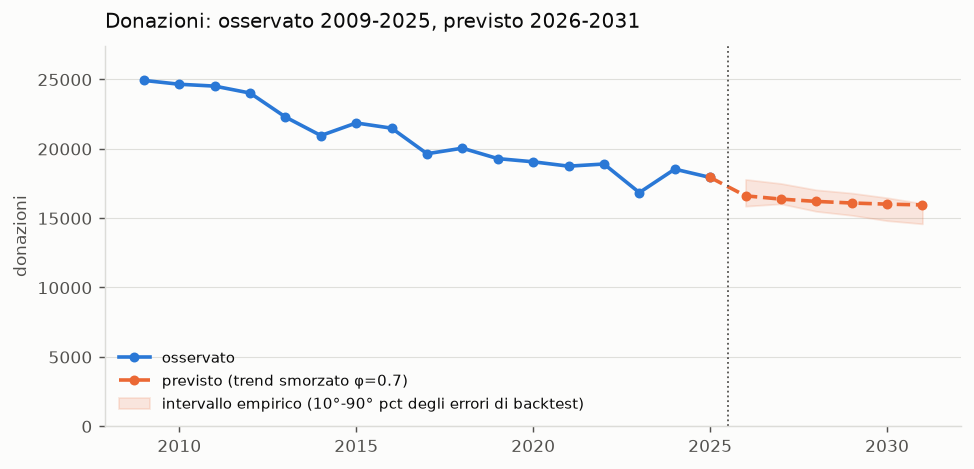
\includegraphics[width=0.95\linewidth]{img/fig_previsione_2026_2031.png}
    \caption{Donazioni annuali osservate 2009--2025 e proiettate 2026--2031}
    \label{fig:fc_forecast}
\end{figure}

\paragraph{Una verifica di coerenza: la somma dei donatori.}
Poiché il panel del \cref{ch:data} materializza gli zeri, è possibile ottenere
la stessa previsione per una strada del tutto diversa: simulare anno per anno
il comportamento di ciascun donatore, aggiungere gli ingressi attesi e sommare.
Il risultato è riportato nella colonna corrispondente di
\texttt{reports/forecast\_2026\_2031.csv}: parte a $+3{,}7\%$ dall'aggregato
nel 2026 e diverge fino al $+15{,}4\%$ nel 2031.

La divergenza è essa stessa un risultato, e ha una causa identificata: il
modello per donatore sovrastima le riattivazioni dal serbatoio dei dormienti,
che cresce di anno in anno perché ogni donatore che smette resta nel panel per
sempre. È la ragione per cui l'appendice adotta la previsione aggregata; ed è
anche un avvertimento sul \cref{ch:glm}, dove lo stesso serbatoio pesa sulle
stime.

% ───────────────────────────────────────────────────────────────────────
\section{Composizione e platea di donatori}
\label{sec:fc_type}

La proiezione per tipologia si ottiene estrapolando la quota di ciascuna
tipologia sull'ultimo decennio e applicandola al totale previsto. L'esito è
negativo: \textbf{la composizione non si muove}. Le quote di
sangue intero, plasmaferesi e aferesi piastrine + plasma restano al 2031 entro
mezzo punto percentuale da quelle osservate nel 2025; in termini assoluti tutte
le tipologie scendono in proporzione al volume complessivo, senza
ricomposizione interna.

L'esito va letto per quello che è: \emph{nulla nei dati recenti segnala una
ricomposizione}, non ``non ci sarà ricomposizione''. L'estrapolazione di una
quota non ha vincoli strutturali e non sa che un cambio di indirizzo regionale
sulla raccolta di plasma potrebbe accelerare bruscamente la transizione.

Quanto alla platea, i nuovi ingressi previsti (con un trend smorzato sulla
serie degli ingressi) scendono da 1\,221 nel 2026 a 1\,162 nel 2031, e
proseguono la flessione già descritta nel \cref{ch:eda}
(\cref{fig:fc_donors}). La lettura, insieme al \cref{ch:retention}, è che la
contrazione attesa è trainata dal lato degli \emph{ingressi} e non da un
peggioramento della fedeltà di chi già dona.

\begin{figure}[H]
    \centering
    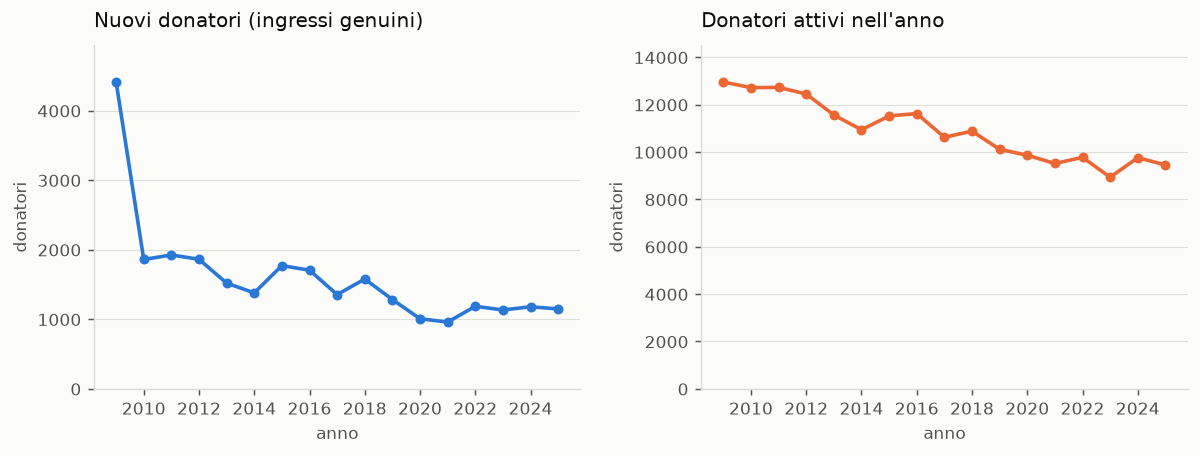
\includegraphics[width=0.95\linewidth]{img/fig_forecast_donors.png}
    \caption{Nuovi donatori (ingressi genuini) e donatori attivi per anno,
    2009--2025.}
    \label{fig:fc_donors}
\end{figure}

% ───────────────────────────────────────────────────────────────────────
\section{Sintesi e limiti}
\label{sec:fc_summary}

\paragraph{1. Flessione lenta, non collasso.}
Circa 97\,200 donazioni complessive nel sessennio 2026--2031, con una
contrazione di poco meno di un punto percentuale l'anno e un valore atteso 2031 di
15\,951 donazioni. Lo scenario è l'assottigliamento lento, non la rottura.

\paragraph{2. Il modello più semplice è il migliore.}
Un trend lineare smorzato batte, sullo stesso backtest, sia le forme a spline
sia i modelli per donatore. La flessibilità paga dentro il campione e costa
fuori.

\paragraph{3. La composizione per tipologia non cambia.}
Nessuna ricomposizione fra sangue intero e plasmaferesi emerge dai dati
recenti.

\paragraph{Limiti.}
\textbf{Proiezioni di tendenza, non scenari:} nessuna proiezione è
condizionata a ipotesi di policy, e una campagna di reclutamento, un cambio di
indirizzo regionale sul plasma o una riorganizzazione dei punti di raccolta
non sono modellati --- i numeri rispondono alla domanda ``cosa succede se
nulla cambia''. \textbf{Gli intervalli poggiano su poche osservazioni:} nove
errori a un anno di distanza, quattro a sei, sono indicazioni, non quantili.
\textbf{La correlazione seriale non è trattata:} nei modelli mensili la
correzione per sovradispersione allarga correttamente gli errori standard, ma
non tiene conto del fatto che mesi vicini non sono estrazioni indipendenti ---
la numerosità efficace è inferiore a 204 e un intervallo calcolato su quella
base resta troppo stretto; servirebbe una covarianza robusta
all'autocorrelazione o un termine autoregressivo esplicito, ed è una delle
ragioni per cui gli intervalli di questa appendice sono empirici. Infine, la
serie contiene \textbf{un evento eccezionale nel periodo di stima}, il 2020:
il suo effetto sul trend di lungo periodo è risultato modesto
(\cref{sec:temporal}), ma la ricorrenza di uno shock analogo non è modellata e
non rientra negli intervalli riportati.

% ══════════════════════════════════════════════════════════════════════════════
%  Fine Capitolo — Proiezioni 2026-2031
% ══════════════════════════════════════════════════════════════════════════════
